\documentclass[pageno]{jpaper}
%%% Local Variables:
%%% TeX-command-extra-options: "-shell-escape"
%%% End:
\newcommand{\Semester}{Spring}
\newcommand{\IWreport}{2018}
\newcommand{\quotes}[1]{``#1''}

\usepackage[english]{babel}
\usepackage{csquotes}
\usepackage{biblatex}

\usepackage{appendix}
\usepackage{titling}

\usepackage{fancyvrb}

\usepackage{minted}
\setminted{baselinestretch=1}

\clubpenalty9998
\widowpenalty9999

\usepackage[normalem]{ulem}

\addbibresource{references.bib}

\begin{document}

\title{
  A Modular Framework for Developing, Deploying, and Evaluating Game-Theoretic Strategy Design Exercises
}

\author{
  Andrew Wonnacott\\
  Advisers: Professor Dave Walker, Professor Matt Weinberg
}

\date{}
\maketitle

\doublespacing{}

\begin{titlingpage}
  \begin{abstract}
    Student interest in ``Economics and Computing'', Princeton's undergraduate computer science course in algorithmic game theory, has grown rapidly in recent years.
    This course employs small simulations to develop students' ability to use theoretical tools to analyze more real-world situations.
    These strategy design exercises require considerably more software infrastructure than a usual theoretical problem set would, including handout code for student self-evaluation and software auto-graders.
    While some frameworks for automated grading exist, none surveyed provided the specific features desired for repeatedly developing very similarly-structured assignments and evaluating student submissions in the context of each other.
    In order to facilitate more automated grading of these assignments in this and future semesters, I have developed a framework of modular, extensible tools for building all of the necessary components of these strategy design assignments.
    Concurrently, in my role as a grader for COS 445, I used the framework to develop and evaluate four strategy design assignments, using assignment specifications developed with Professor Weinberg.
    This provides feedback from real student and instructor users, which was then used to improve the auto-grader design.
    Empirical results demonstrate the importance of quality tooling to effective use of instructor time, low broken submission rates, and high student satisfaction.
  \end{abstract}
\end{titlingpage}

\section*{Introduction}
My work builds upon existing programming-based game theory exercises assigned in Princeton's COS 445 ``Economics and Computing''.
The intention of these strategy design exercises is to teach students how to use game theory to analyze a real-world situation and work rationally within a healthy incentive structure, e.g.\ one in which students do not try to hurt each others’ performance.
Each past offering of the course has rebuilt these assignments, and all associated instructor tooling, from scratch, resulting in unnecessarily high allocation of instructor time to grading.
Additionally, the course has grown rapidly to become the single largest theoretical computer science course ever taught at Princeton~\cite{coursesizes}.\footnote{More students complete COS 340 in a given year, but it is taught in both fall and spring semesters.}

The goals of this project are to discover to what degree the development of new strategy design exercises can be simplified or automated, to improve the student resources available during the completion of these exercises, and to create institutional memory and decrease year-to-year repetition.
This was accomplished by designing a modular, extensible, and reusable framework which embodies the commonality between strategy design exercises, allowing instructors to create new exercises while changing only the necessary, assignment-specific details, by developing more advanced automated grading tools than previously existed for the course.
Within this framework, I have built a collection of utilities to facilitate students' evaluation of their own strategies and to decrease strategy iteration overhead.

Through this work, I aim to improve the quality of computer science theory education from the perspectives of both the students and faculty associated with COS 445.
Quantitative metrics, including software failure rates and instructor time usage, and qualitative metrics, including student and instructor satisfaction, both illustrate the improvements to the course and emphasize the importance of quality tooling to quality programming-based assignments.

\section*{Problem Background}
Four Princeton University departments offer courses in game theory: Economics, Politics, Mathematics, and Computer Science.
While all of these courses teach the core concepts of game theory, each also connects this core to relevant examples and topics in its department.
For instance, the Computer Science department's ``Economics and Computing'' places emphasis on the connections between game-theoretic results and algorithms, software, and other aspects of computer science.
The course focuses on the relevance of game theory to matchings, auctions, cryptocurrencies, and other multi-actor computational systems~\cite{cos445sp18}.
It is also represented in the design of the problem sets, which, in addition to traditional proof-based exercises, contain programming-based exercises which connect course topics to prerequisite computer science skills.
These programming-based exercises take a common form.

Students are presented with an iterated game, described both in the assignment handout and as a Java interface.
A classic iterated game is the iterated prisoner's dilemma, as in Figure~\ref{fig:pd},
\begin{figure}[hbt]
  \centering
  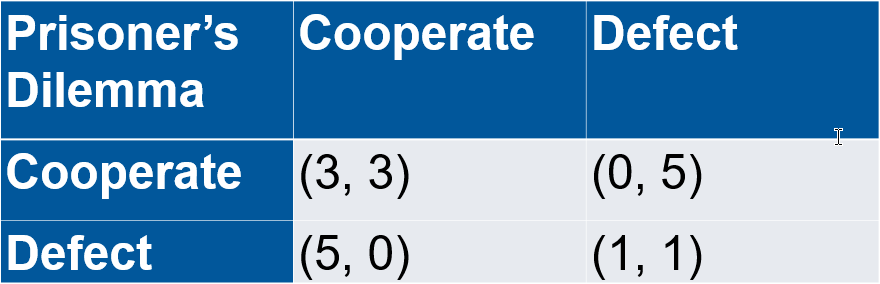
\includegraphics[scale=0.5]{pd.png}
  \caption{The payoffs of each round of the iterated prisoner's dilemma.}\label{fig:pd}
\end{figure}
in which two players must collaborate to receive the best outcome and have access to the other player's previous decisions when making their own decision.
Players balance the incentive to defect, which improves their own situation while damaging their opponent, with the knowledge that their opponent may defect in future rounds punish them if they defect now.
This game translates to the interface in Figure~\ref{minted:Prisoner}.
\begin{figure}[hbt]
\begin{minted}{java}
    public static <Student_T extends Student> int[] withExtraTrial(
            Class<Student_T> clazz, double S, double T, double W)
    {
        // Initialize students
        Student[] students = new Student[N+1];
        //R students[{0}] = new Student_{netID}();//
        try {
            students[N] = clazz.getConstructor().newInstance();
        } catch (ReflectiveOperationException roe) {
            roe.printStackTrace();
            System.exit(1);
        }

        return runTrial(students, S, T, W);
    }
\end{minted}
  \caption{\texttt{interface Prisoner} demonstrates a strategy interface}\label{minted:Prisoner}
\end{figure}
While this game is well-studied and models some real-world incentive structures, the course also draws on various real-world phenomenon to design iterated games, including a college admissions game from the perspective of stable matchings, a search advertisement bidding game using auction theory, an election informed by voting theory, a gerrymandering-prevention simulation inspired by fair division, and exploitation of a fictional cryptocurrency by analyzing blockchain incentives.
These examples are not exhaustive, but illustrate the variety of course topics with potential for translation to iterated games.

Students then craft strategies to play the specified game, based on their own analyses of the game's equilibrium and on which strategies they expect their peers to submit.
These strategies are evaluated on both on their design quality and on their empirical performance.
While design quality is evaluated on a purely individual basis, empirical performance is measured by simulating the play of the collection of submitted student strategies against each other.
For instance, for the iterated prisoner's dilemma, every student strategy plays one `full' game, consisting of many iterations of the prisoner's dilemma, against each other student strategy.
Strategies are scored based off the average payoff they achieve.
For the search advertisement game, all the student strategies are concurrently asked to bid on the same search terms.
They are scored based on their revenue from ad clicks minus their expenditures on advertising, and each bidder knows the click-through rate for a term prior to bidding on that term.
To create a more realistic simulation, students are graded solely on the performance of their own strategy, not on a curve of the performance of their peers.
That is to say, student grades on these strategy design exercises are not zero-sum.

These strategy design exercises are intended to help students place theoretical results from the course in context.
They create a scenario in which mastery of theoretical course content is demonstrated by making and justifying real-world decisions.
Professor Weinberg's intent is that no student should experience difficulty implementing their strategy, and all of the challenge should come from developing a creative, successful strategy.

While the strategy design exercises assignments are popular with students~\cite{cos445sp17review}, they also demand dedication of considerable instructor resources to building software for student handouts and strategy evaluation, which have historically been significantly rebuilt for each assignment.
Worse still, due to course staffing changes, this work has not been preserved between semesters, resulting in inefficient allocation of department resources to producing new exercises without the institutional memory or software resources previously developed.
Due to the limited tooling provided in past semesters for students to test their code, many submissions did not compile or caused run-time exceptions, requiring considerable additional instructor resources.


\section*{Related Work}
This work was developed to replace previous software design exercises assigned to COS 445 students\footnote{including the author} in Spring 2017~\cite{cos445sp17}.
In one problem set, students developed and implemented strategies for three different strategy design exercises related to three different abstract games: Prisoner's Dilemma, Centipede, and Ultimatum.
In a later problem set, an exercise placed students in the role of bidders in a generalized second-price auction.\footnote{A G.S.P.\ auction is an auction of multiple items, one after another, where the winning bid pays the second highest bid. This is the auction format used by Google to sell sponsored search auctions.}

Both problem sets were implemented and graded by Cyril Zhang~\cite{cyrilzhang}, a graduate student TA for the course.
Zhang developed interfaces, dummy implementations, and grader software for each strategy design exercise~\cite{s17}.
However, his implementation of software for strategy design assignments was intended for grader use only.
It is not modular and has to be completely rewritten for each assignment.
The student interfaces were documented, but the grader software was not documented for future use.
Additionally, some of the scripts and notebooks used by Zhang were not preserved and were not accessible as resources.
Thus, while these resources served as inspiration for this work and provided some assignment-specific code to my work developing specific assignments, I did not build directly on Zhang's code.

Prior to Spring 2017, COS 445 was taught by Professor Mark Braverman in Fall 2012 and Spring 2014~\cite{coursehistory}.
Though no documentation or archives of the course homepage from these semesters is available online or in the Internet Archive, I recovered some resources from the course account on the ``Cycles'' cluster of the Princeton Computer Science department and from the source code repositories used by the course staff.
In both semesters, Yonatan Naamad~\cite{ynaamad}, a former graduate student TA for the course, was responsible for software development.

The only resources available from Fall 2012 were collected from the course Google Code repository~\cite{googlecode}.
This repository contains incomplete Python skeleton code for a basic tournament of an unspecified game.
I uploaded this code to the current course repository~\cite{f12} but did not develop it further.

The Spring 2014 iteration of the course was developed on a private GitHub repository at ynaamad:cos445, which I am unable to access directly.
Through a clone of this repository stored on Cycles, I discovered that the course had PHP and Java implementations of strategy design exercises for Prisoner's Dilemma and another auction setting.
The Java code was the student handout, which contained strategy interfaces and some testing code.
The testing code was not designed to be automated for grading and was not modular.
It tested manually-entered strategies against each other, and assignment-specific details such as game structure and payoffs were integrated within the simulation code.
As a design decision I dismissed the available PHP code, which was used for course grading, due to language unfamiliarity.
These resources were uploaded to the current course repository~\cite{s14}, but were not reused, in part because they were located and examined only when I was given access to the course site in order to deploy my project.

Beyond COS 445 at Princeton, many universities have taught computer science courses in algorithmic game theory.
However, a survey of several universities' courses, including courses at Harvard~\cite{harvard}, Stanford~\cite{stanford364a}~\cite{stanfordf16}, Cornell~\cite{cornell}, U.\ Washington~\cite{uw}, Yale~\cite{yale}, U.\ Penn~\cite{penn}, Georgia Tech~\cite{gtech}, MIT~\cite{mit}, Carnegie Mellon~\cite{cmu}, and Duke~\cite{duke}, identified only one other course with similarly-structured assignments.

Harvard's Computer Science 136, ``Economics and Computation''~\cite{harvard}, assigns two programming problem sets.
The first requires implementation of a peer-to-peer file sharing system similar to BitTorrent, a protocol in which incentives parallel Prisoner's Dilemma.
However, the assignment is not a competition and student solutions are not differentiated based on strategic properties.
The second assignment is a strategy design exercise built on the generalized second-price auction, in which student strategies vary and are graded based on their performance in a competitive environment.
This is very similar to both the Spring 2014 and Spring 2017 auction exercises of COS 445 at Princeton.
However, the grading structure of this assignment is quite different from the grading structure of the COS 445 strategy design exercises, and the implementation is in Python.
While comparison between COS 445 assignments and CS 136 assignments in a future project might provide some pedagogical value, such work would be out of scope for this project.
Given that these assignments are implemented in Python, only handout (and not grading) code is available, and the assignments are graded differently, these resources were dismissed as a base for development of new resources for COS 445.

Many universities, including Princeton, maintain extensive systems for the automatic submission and processing of student assignments.
Such resources are useful in the general case of developing new programming-based assignments, but no such resources replicate the behavior implemented in this project.
Most auto-grading systems are designed with an assumption that each student submission is graded in isolation from other student submissions.
Such systems are not applicable to this project since the strategy design exercises involve evaluation of student strategy performance in a common environment.
Though existing automatic grading systems cannot replicate the full extent of this work, I have integrated existing resources for assignment submission and student feedback to perform smaller tasks within a larger system.
I integrated CS DropBox~\cite{csdropbox} functionality where relevant, and I modeled the leaderboard structure after review of the leaderboard implementation used in other Princeton CS classes.
Generally, no such tools would leverage the high degree of structural similarity between strategy design exercises, and a dedicated project for these exercises will allow for more efficient development and evaluation.

\section*{Approach}
Cyril Zhang completed the TA requirement for the PhD program last fall, so at the start of this semester it was unclear who among the graduate and undergraduate course staff would be responsible for maintaining the COS 445 strategy design exercises.
Therefore, the course needed not just long-term work to improve student and instructor resources, but also short-term work to maintain and debug the same resources.
These coinciding requirements inspired me to design one extensible implementation of all the reusable components for software design exercises, and to develop the project iteratively in conjunction with its usage in the course.
This software would naturally grow throughout development as demanded by the needs of the course, and the final product will naturally lower-bound the maximum degree of automation and modularity possible.
While this decision to develop my software using agile methods obviates the need for an extensive design process, a few key decisions were still needed before implementation could commence.

While I was initially inclined to pursue implementation in Java, I spent considerable effort on language selection to verify this decision.
This was necessary because I would incur a considerable cost to myself and to others ere I to change programming languages partway through the semester.
I would have to rebuild all previous work, and I would inconvenience all the students of COS 445 by making them change languages and wasting their time learning the abandoned language.

Many students suggested the assignments be implemented in Python~\cite{survey12, survey34}, and this would be preferred by the course staff as well.
Members of the Mechanism Design group are not expected to have working proficiency with Java, but many have enough experience with Python to support students.
Additionally, Python's conciseness and ability to load classes from user input would be useful when implementing tools which are parameterized on user-input strategy names.
Unfortunately, COS 445's prerequisite courses only provide Java experience, and not Python experience, so students reasonably expect they will only be asked to write Java code.
Data from other course surveys (Appendix~\ref{appendix:cos333sp17}, Appendix~\ref{appendix:cos333sp18}) indicate that 90\% of students report themselves fluent in Java after the Princeton introductory sequence, compared to 30\% for Python, confirming that the student work for the assignment must be in Java.
Given this constraint, and lacking any other language selection pressures, I elected to implement as much of the assignment code as possible in Java, with limited usage of scripting languages such as Python, Bash, and GNU Make.
These scripting languages were used only where Java would not suffice and only where implementation details were irrelevant to student assignment comprehension.

Java also offers convenience to assignment designers by enforcing an object-oriented design pattern.
This allows instructors to communicate assignment specifications formally through a well-documented interface.
Furthermore, by constructing new instances of student implementations between game rounds, instructors can programatically enforce that students do not employ learning strategies outside the parameters of the assignment.\footnote{This requires that instructors forbid the usage of static variables, but it is trivial to verify compliance with this requirement.}

However, several default Java behaviors do not map cleanly onto the desired properties of strategy design exercises.
For instance, Java objects used as function parameters are passed by mutable, nullable reference.
This is in contrast to functional languages (including Ocaml and Rust), where parameters are immutable and non-null unless otherwise explicitly specified.
Current industry standards for Java code obviate both of these issues using modern language features~\cite{guavanull, guavaimmutable, unmodlist}.
In order to preserve backwards compatibility, these features are not implemented by default.
Where possible, I have taken advantage of these features.
Since the assignment specification documents that students are required not to modify parameters, instructor code can use unmodifiable (immutable) containers.
However, I have not included \texttt{NotNull} annotations because they are not taught in the prerequisite courses and, as previously noted, these assignments should not require students to self-teach any programming skills.
In my own framework code, which must be supported by future instructors, I decided to assume support for Java 9, released in fall 2016~\cite{techworld}, and to use modern language features, since course instructors are at least as likely to have industry experience with modern Java code as experience with the Princeton introductory sequence.

While of lesser urgency, I have also planned ahead to ensure the re-usability of my work.
I elected to store this work in a University-owned private GitHub repository.
I also documented the repository structure and contents, including a summary of the process of developing and deploying a new assignment.
This ensures that future course staff will have the physical and technical means to maintain this project after I have graduated.

\section*{Implementation}
Before the first problem set of the course was assigned in this semester, Professor Weinberg and I designed a handout interface and tools to allow students to test their strategies against each other, which I then implemented.
The game simulates college admissions using stable matchings.
While I implemented this handout with the explicit goal of producing a tool to test out multiple different student strategies in the specified application environment, I followed the principles of modular software design taught in COS 217~\cite[Chapter~4]{tpop99}.
I factored out the code which implemented the Gale-Shapley deferred acceptance algorithm for stable matchings from the code which performed randomized trials of the stable matchings and produced performance statistics for students.

When it came time to implement the second strategy design exercise, I was able to reuse code which processed results of trials, even though the nature of the trials changed from college admissions to elections.
Additionally, when it came time to grade the problem set, I was able to modify only the post-processing step to compute grades.
Thus, creating a new assignment required constant work in the number of framework extensions, while creating a new framework extension requires constant work in the number of assignments.
The result of this process duplicates significant functionality from last year's assignments.

However, because of conscious design decisions to factor out repeated code within each assignment, my project will be more reusable than implementations from past semesters.
It is also extensible, so new extensions such as additional tools or interfaces can be written for strategy design exercises.
The structure of my project is outlined in Figure~\ref{fig:outline}.
The modular layout ensures that each component can be designated as either reusable between assignments (green), written for each assignment by the instructors (blue), or submitted by each student for each assignment (orange).
Throughout the semester, I have leveraged my role as an undergraduate course assistant for COS 445 during the current semester in order to identify and produce extensions, including CS Dropbox ``Check Submit'' functionality and a student strategy leaderboard.
This framework reusable, both for the same assignments in future years and for new strategy design exercises implemented by future course staff with lower overhead.

\begin{figure}[hbt]
  \centering
  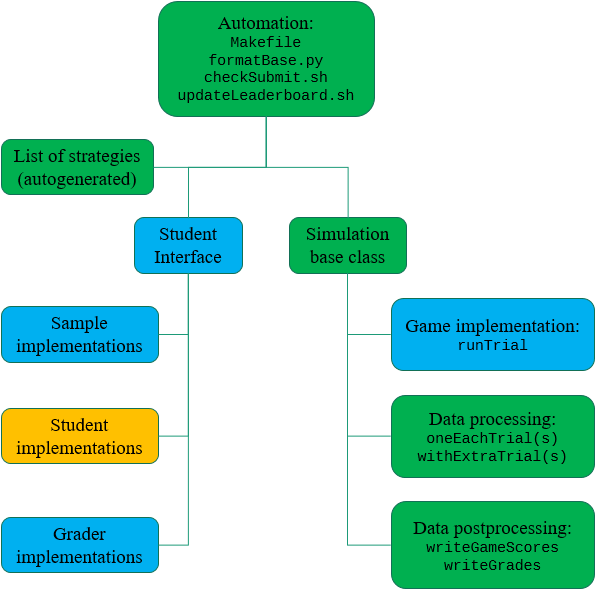
\includegraphics[scale=0.75]{outline.png}
  \caption{The implementation structure of my framework.}\label{fig:outline}
\end{figure}

\subsection*{Handout Implementation}
In order to design my framework, I reviewed non-modular code from the Spring 2017 auctions exercise.
This is the only assignment for which I had access to both the student handout and the grader code.
In any strategy design exercise, after the game design is complete, the next step is to implement is the student interface.
The interface for the auctions exercise is quite simple, as shown in Figure~\ref{minted:Bidder}.
\begin{figure}[hbt]
\begin{minted}{java}
import java.util.List;

public interface Bidder {
    // Return your bid for the current day
    // Called once per day before the auction
    public double getBid(double dailyValue);

    // Let you know if you won, and how much the winners paid
    // Called once per day after the auction
    public void addResults(List<Double> bids, int myBid, double myPayment);
}
\end{minted}
  \caption{\texttt{interface Bidder} demonstrates a strategy interface}\label{minted:Bidder}
\end{figure}

This interface describes the necessary functions of a student strategy for the auctions exercise.
Each day, they must bid on an auction of advertising slots which appear on a search results page (often called ``sponsored search results'') and assign different values to words auctioned on different days.
The strategy also has access the winning bids for each of the ten sponsored results from each past day and knows which of those bids were its own.\footnote{When a strategy wins, it is also told how much it paid.}
This allows the strategy to obey the budget constraint: across all 1000 days, it may not spend more than 500.
These constants are not documented in the interface as designed, only in the assignment specification.
The instructors distribute a simple sample student implementation --- in this case, the truthful bidder.
Zhang also implemented a program used to grade the student-submitted strategies which consisted of two methods: \texttt{main} and \texttt{trial}.
The former ran 100 trials and printed out the results, averaging the outcomes across each trial for each student.
The latter contained an implementation of the generalized second-price auction format described in the assignment specification.

Having reviewed a former assignment, I implemented the first assignment handout for the course this semester: the college admissions simulation described previously.
In doing so, I made several implementation decisions in order to facilitate future reconfiguration of both the game being played and the post-processing of tournament results, which are representative of design decisions made throughout the assignment.
In every assignment, the tournament simulation portion (instructor-written code) is broken up into game rounds, result processing and amortization, and further post-processing, such as grade assignment and output formatting.
The divide between game rounds and code which processes game results was present in Zhang's auction code as the separation between the \texttt{trial} and \texttt{main} methods.
However, this prior work did minimal amortization and no advanced output formatting, and had no separation between them.
While the handout code written for the first assignment did minimal post-processing, this distinction was quite useful when later developing the auto-grader and additional extensions.

During the development of this handout, however, the statically-typed nature of Java raised some difficulty.
Zhang's grader code had student submission names hard-coded into complex expressions, as though they had been copied in from a manually-written list formatted using \texttt{sed}.
In the context of developing a handout to allow students to test multiple strategies of their own design, I determined that requiring students to modify the simulator Java code whenever they changed which strategies they wanted to test would be so cumbersome that the simulator might not have been distributed at all.
Additionally, graders desire functionality to configure the list of evaluated strategies without having to manually list out all the student strategy names and modify it to identify and diagnose misbehaving student strategies.
Since Java is not able to type-check user-input strategy names, I determined that the most effective workaround for this issue would be to automatically rewrite the Java code before compile-time.

For this purpose, I developed a simple Python script capable of rewriting arbitrary template plain-text files using a CSV file.
This script, \texttt{formatBase.py}, included as Appendix~\ref{appendix:formatBase}, builds a list of dictionaries, one for each row of the CSV, using the header of the CSV as the keys and the contents of the row as the values.
In its input, it identifies lines which start with \texttt{//R} and end with \texttt{//}.
For each such line in its input, it outputs multiple lines, each corresponding to the input line rewritten using a distinct row of the CSV by replacing each curly-enclosed key with the corresponding value.
It also rewrites the key \texttt{0} with the row number from the configuration table.
This script directly injects the contents of the configuration file into the Java code with no escaping, as is necessary in this application.
However, this practice is extremely dangerous, since using a user-submitted configuration file would allow users to execute arbitrary code on the evaluation machine.
Fortunately, this is not a security concern, since students already run arbitrary code on the evaluation machine: their submitted strategy.

Given a CSV file as input with the header row \texttt{netID} and a row for each student's name, the method in Figure~\ref{minted:oneEachTrial} will be rewritten to instantiate one object of each Student implementation listed in the configuration file:
\begin{figure}[hbt]
\begin{minted}{java}
    // S, T, W are simulation parameters documented in the student interface
    public static int[] oneEachTrial(double S, double T, double W)
    {
        // Initialize students
        Student[] students = new Student[N];
        //R students[{0}] = new Student_{netID}();//
        return runTrial(students, S, T, W);
    }
\end{minted}
  \caption{\texttt{oneEachTrial} demonstrates usage of \texttt{formatBase.py}}\label{minted:oneEachTrial}
\end{figure}
My modular design allows for data collection code to vary without additional overhead.
This is shown in Figure~\ref{minted:withExtraTrial}, which instantiates an instructor-provided strategy using reflection, in addition to the strategies specified in the configuration file.
This method is useful for grading assignments.
\begin{figure}[hbt]
\begin{minted}{java}
    public static <Student_T extends Student> int[] withExtraTrial(
            Class<Student_T> clazz, double S, double T, double W)
    {
        // Initialize students
        Student[] students = new Student[N+1];
        //R students[{0}] = new Student_{netID}();//
        try {
            students[N] = clazz.getConstructor().newInstance();
        } catch (ReflectiveOperationException roe) {
            roe.printStackTrace();
            System.exit(1);
        }

        return runTrial(students, S, T, W);
    }
\end{minted}
  \caption{\texttt{withExtraTrial} demonstrates modularity in data processing}\label{minted:withExtraTrial}
\end{figure}

Given all of the components described above, I have developed a considerably improved the assignment handout.
Previously, the handout contained the strategy interface and a simple implementation strategy with a sample testing method for that implementation only.
This semester, assignment handouts contained not just the strategy interface and simple implementation, but also a full copy of the above game round simulation, complete with amortization by many randomized trials, which simply prints the average score of each strategy.
While working on the assignment, students can reconfigure the testing code easily by modifying the configuration file to contain whatever strategies they want to simulate.
For instance, given strategies \texttt{Student\_random.java} and \texttt{Student\_favorites.java}, which apply to random schools and favorite schools in the above college admissions simulation, all the student would need to do to simulate ten submissions using the former strategy and 15 using the latter would be set the configuration file to ten lines of \texttt{random} and 15 lines of \texttt{favorites}, and then run \texttt{make test}.
Such a configuration file is included as Appendix~\ref{appendix:students}.
Whereas last year each student would have had to manually write simulation code to run the exact collection of strategies they wanted to simulate, the new handout will automatically rewrite the simulation code to simulate those strategies using \texttt{formatBase.py} and then compile and run the simulation with no additional overhead.

\subsection*{Auto-Grader Design}
The two most important components of each exercise are the handout code for the students and the auto-grader code for the instructors.
However, in order to design the auto-grader, Professor Weinberg and I had to develop a well-specified, portable standard for grading strategy design exercises.
A key constraint in the grading of these assignments is that the students must be incentivized to maximize their own strategy's performance, and not incentivized to either help or hurt their peers except when doing so helps themselves.\footnote{Of course, students are encouraged to help their peers out of their own compassion, and doing so contributes to their course participation grade, but they are not rewarded for doing so in their assignment.}
Therefore, curving each student's grade based on the percentile of their strategy's performance is not acceptable.
In this scenario, a student would be as happy to hurt their peers as to improve their own strategy.
For instance, in an iterated prisoner's dilemma, if students are graded based on relative performance, then they are apathetic between both cooperating and both defecting.
So there is no incentive under any circumstance to cooperate, even in the face of potentially irrational counter-parties, and every student should always defect.

One feasible grading strategy, given this constraint, would be to grade student performance without any curve at all.
That is, in a simulation where the best possible performance is 5000 points, and the worst possible performance is 0 points, students would receive 3/5 on the assignment if they scored 3000 points on average.
However, in this case, student grades can be negatively impacted by the decisions of their peers.
For instance, in the prisoner's dilemma, for every student who always defected, every other student would have the cap on the maximum possible grade they could receive lowered.
Students' grades would be dominated not by the performance of their own strategy but by the decisions of their peers.
Course staff, including Professor Weinberg, agreed that this is unacceptable.

``Replacement-comparison grading'', the grading rubric used in the course, was developed by Professor Weinberg and myself as a dependency of my work on this project, and satisfies the need for an incentive-correct grading rubric which could be implemented in an auto-grader.
It is based on the following intuition: to grade a given student's strategies in a room with their peers, substitute each instructor in their place while making no other changes to the room, and measure whether the student does better or worse than that instructor would have in their place.
The performance of a student strategy $S_i$ among strategies $S_1 \ldots S_n$, pro-rated based on the potential best and worst possible performances by any strategy in the simulation can be captured by comparing the score $x_i$ of $S_i$ against $S_1 \ldots S_{i-1}, S_{i+1} \ldots S_n$ to the scores $y_{i,1} \ldots y_{i,m}$ of a predetermined menagerie of $m$ instructor strategies $I_1 \ldots I_m$, where each $y_{i,j}$ in $y_{i,1} \ldots y_{i,m}$ is the score of $I_j$ against $S_1 \ldots S_{i-1}, S_{i+1} \ldots S_n$.
Students whose strategies outperform all instructor-designed strategies have done better than the instructors would have at the assignment, and receive the best grades.
Some instructor-designed strategies are intentionally imperfect or misguided, in order to differentiate between less ideal student-designed strategies.

This grading strategy has the correct incentives: each student will work to maximize their chance of beating each instructor threshold, not to sabotage their peers' performance.
Since the instructor strategies used for grading are not revealed and the pool of other student submissions is unpredictable, the distribution of instructor thresholds approaches uniform, and students will attempt to beat as much of the real interval of the score range as possible, producing the same behavior as students maximizing expectation.
Additionally, by amortizing student performance over many randomized trials --- for instance by reassigning student and university preference orderings in the college applications game independently between trials --- the law of large numbers guarantees to students that their grade represents their expected performance without uncertainty based on variance between trials.
Thus, students are not incentivized to play a lower-expectation strategy in order to increase their variance.\footnote{The same analysis holds for all higher moments of their strategy.}
This system is also not vulnerable to students attempting to sabotage instructor scores for their own benefit, since instructor scores for a given student are calculated without the play of this student.

Though the above strategy achieves all the correctness requirements, it has a fatal flaw: when there are $n$ student strategies and $m$ instructor strategies, and a trial with $n$ strategies takes $t(n)$ time, this grading metric takes $O(m \cdot n \cdot t(n))$ time.
After approval from Professor Weinberg, I implemented a simple optimization to bring down the time requirement to $O((m+1) \cdot t(n+1))$ time.\footnote{So long as $t$ grows slower than $n! $, this is a performance improvement; for practical reasons, all simulations used in this course take polynomial time in the number of students.}
The modified replacement-comparison grading scheme measures student scores $x_1 \ldots x_n$ for all students $S_1 \ldots S_n$ amortized across many trials, and then measures $y_j$ against all of $S_1 \ldots S_n$ for each instructor strategy $I_j$ among $I_1 \ldots I_m$.
That is to say, instructor strategies are assigned $y_j$ based on their performance against all the students, while student strategies are assigned $x_i$ based on their performance against all the other students.
Student grades are still assigned based on how many instructor strategies performed worse than their strategy, computed as $\sum\limits_{i=1}^n \delta_{x_i > y_j}$ as before.

The only difference between the initial and modified replacement-comparison schemes is that each student can have some small impact on the thresholds used to grade themselves, not just their peers.
As an unfortunate consequence of this simplification, if a student was able to hurt instructor scores, they might perform better.
However, since students cannot identify when they play against an instructor, as opposed to a peer, they must do so by playing to sabotage all their peers' scores.
When multiple students try to sabotage instructor scores, they also sabotage each other, and all student scores will be correspondingly lower.
In this situation, the damage to the grader strategies' scores is representative of lower potential performance by any student strategy.
Thus, the modified replacement-comparison scheme is sufficient.

\subsection*{Auto-Grader Implementation}
The goal of this project is not just to build a handout and an auto-grader, but to build a framework in which the development of the grader as described above requires no modification of assignment-specific code.
Consider the components of the simulation handout:
\begin{itemize}
\item
  \texttt{runTrial} method which takes a list of strategies and simulates their behaviors, e.g.\ in a college admissions simulation
\item
  data processing methods, e.g.\ \texttt{oneEachTrial} (Figure~\ref{minted:oneEachTrial}), which builds a list containing each configuration-specified strategy once, and \texttt{oneEachTrials} (not shown above), which runs \texttt{oneEachTrial} a large number of times and averages the results
\item
  post-processing methods, e.g.\ outputting a CSV file containing student names and their average performance in the simulation
\end{itemize}

Only the first of these contains assignment-specific code.
In order to implement replacement-comparison grading, I implemented the following methods:

\begin{itemize}
\item
  two new data processing methods: \texttt{withExtraTrial} (Figure~\ref{minted:withExtraTrial}), which builds a list containing each configuration-specified strategy once, and one extra strategy passed in as a parameter, and a corresponding method \texttt{withExtraTrials}, which averages the above.
  These are very similar to the existing data processing methods
\item
  A new post-processing method that computes grades for each student given how many instructor strategies each student strategy outperformed and a lookup table to translate this win-count to an assignment grade.
  This method, \texttt{writeGrades}, is included as Appendix~\ref{appendix:writeGrades}
\end{itemize}

Given only these two changes, the handout code has been transformed into an auto-grader.
Additionally, neither of these changes required alteration of the \texttt{runTrial} method, so minimal additional work is necessary for grading an assignment once the handout has been made.
Only filling in the instructor strategy names and scoring rubric is needed.

In summary, as described in Figure~\ref{fig:outline}, each assignment consists of a strategy interface, implementations of that strategy, a list of those implementations, a \texttt{runTrial} method which specifies how to evaluate those strategies, methods which run specific subsets of strategies, methods that post-process the results of those trials to provide low-latency feedback or for auto-grading, and automating these steps with a Makefile to configure, compile, and run the assignment simulation.

In addition to easily altering an assignment handout into an auto-grader, my framework also makes it easy to build new assignments.
To adapt the college admissions exercise described above into the elections simulation of the second problem set of COS 445 this spring, only a few changes were necessary.

Specifically, I had to develop changes only to assignment components which were not modified between the handout and the grader.
The written assignment specification describes a new strategy format, so a new Java interface file was necessary.
Of course, all the implementations of this interface were also written from scratch for the new assignment, all of which are fairly concise but express assignment-specific strategies.
Finally, the \texttt{runTrial} method of the simulator had to be rewritten to simulate an election instead of college admissions.
No semantic changes were necessary to the data processing or post-processing methods for either the handout or application.

\subsection*{Development of Further Tooling}
As currently implemented, each assignment was distributed as a standalone zip file through the course website.
Even though significant code was shared between the two assignments described above, they were distributed as separate files.
While further modularization would allow code that changes each assignment --- describing how to simulate a game round --- to be separated out from code which changes between the handout and the auto-grader, I determined during assignment development that maintaining separate code bases for each assignment has significant advantages.
Some simulation parameters, such as the budget constraint or number of auctioned items in an auction, vary between assignments.
Often, strategies are evaluated based on their performance relative to baseline instructor strategies in several different regimes of simulation parameters.
This will involve tweaks to the grader code outside of the scope described above.
While these changes are minimal and necessary, keeping details of grading separate between assignments proves useful in the real world.

Thus far, I have illustrated the strengths of my project at performing tasks which were envisioned from the outset.
The strength of modular implementation also comes from the ability to adapt to changing demands easily in real time.
In this way, I was able to extend my framework throughout the semester in order to address my needs as a course assistant to remedy issues with the strategy design exercises.
While the handout code enabled students to verify that their code compiled and ran on their own personal computers, several students submitted non-functioning strategies due to environmental differences, demonstrating the classic issue ``Works On My Machine''.

Other computer science courses at Princeton employ an online tool in the CS Dropbox called ``Check Submit''.
This tool allows instructors to specify tests to be run on department-configured machines using student code, and enables students to evaluate the performance of their submission against these tests without the concern that the software environment on their machine might not be compatible.
I enabled ``Check Submit'' for COS 445 strategy design exercises as a part of this work by developing simple Bash script and Makefile which adapts my assignment framework to this new setting.
My ``Check Submit'' script copies in the assignment handout from a predefined location into the student submission folder, detect the student submission name, and write the \texttt{formatBase.py} configuration file to run their submission.
Now, without any modification of the assignment code, every strategy design exercise automatically has Dropbox ``Check Submit'' functionality possible.
This confirms to students that their strategy will not be incompatible with the grading environment, improving student satisfaction with the course.

However, students would still benefit from more realistic testing.
Thus, I developed a leaderboard so students could better understand how a strategy would perform against more realistic collection of peer strategies.
First, I initialized a new Dropbox assignment for students to submit strategies to the leaderboard, though these strategies need not be their final assignment submission.
I implemented the leaderboard by writing a simple Bash script which scrapes all student submissions from the Dropbox, automatically writes the configuration file to run every students' submission together, and runs the simulation provided in the student handout as above.
Because the simulation output is an easy-to-parse table, I can automatically reformat it into an HTML table and place this in a web page accessible through the department web servers.
The script to update the leaderboard runs through a \texttt{cron} job at a customizable interval.

While this leaderboard provides additional feedback, there are unavoidable issues when students submit broken code.
Since all student submissions are run together, one non-compiling or exception-throwing submission disables the leaderboard for all students.
I worked around this issue by disabling assertions, which were used in \texttt{runTrial} to automatically halt simulation whenever a student submission performed behavior in violation of the assignment specification.
With this modification, the code automatically falls back to silently overriding illegal values from student strategies with sane but selfless defaults so that the leaderboard is correctly generated even when some student submissions are faulty.
Some student code also caused compilation failures, which are more difficult to work around.
We enabled the ``Check Submit'' button to leaderboard so that students could check their leaderboard strategies would compile in the department environment.
This mostly resolved the issue.

\section*{Results}
This project has already achieved minimum viable product by providing a framework for implementation of strategy design exercises in the current year of COS 445.
These assignments and the framework I developed are documented and available at the course GitHub site~\cite{s18}.
Thus, they will be available for reuse in future offerings of the course.

While I have been unable to experimentally determine whether my project will be reused, I have evaluated my successful achievement of each other goal.
I have decreased the work to build each assignment within a semester and the instructor time allocated to assignment implementation, eliminated the inter-year assignment reconstruction, and improved available student resources.
These achievements have increased student and instructor satisfaction with the strategy design exercises.

My primary goal, which unifies my work and sets it apart from past work on this subject, has been to discover modularity and decrease assignment-to-assignment rewriting.
As measured using \texttt{cloc}, development of the fourth strategy design exercise required only TODO\% of the code be modified from previous assignments~\cite{s18}.\footnote{TODO lines of code be changed out of TODO lines of code total assigned or graded.}
As illustrated in Figure~\ref{fig:instructortime}, which shows each assignment from Spring 2018 in chronological order, instructor time usage dropped radically with each exercise, demonstrating the benefits of modular design.\footnote{This data is exaggerated by the overhead of modularization and includes time spent on framework development where that was a direct dependency of instructor work.}

\begin{figure}[hbt]
  \centering
  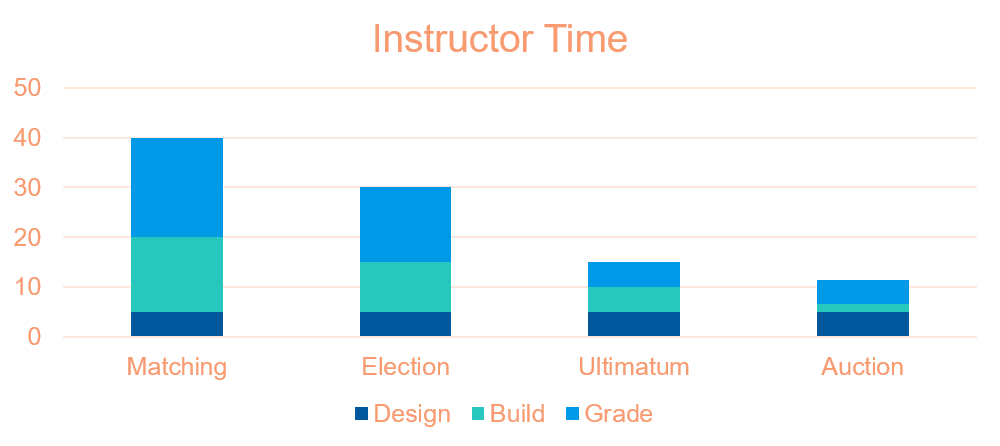
\includegraphics[width=0.75\linewidth]{instructortime.png}
  \caption{Instructor time usage dropped radically as my framework was deployed. (Table~\ref{table:time})}\label{fig:instructortime}
\end{figure}

I have also succeeded at leveraging the extensibility of my project to improve student resources.
As measured using \texttt{cloc}, the ``Check Submit'' button required 28 lines of code and the leaderboard required 34 lines of code to implement~\cite{s18}, representing roughly 15\% each of the size framework developed previously.
With these remarkably simple extensions, student performance improved dramatically.
``Illegal submissions'' constitute student strategies which do not compile, throw exceptions, violate assertions, or otherwise behave outside of the parameters of the simulation.\footnote{Poorly performing strategies which obey the specification are legal.}
The illegal submission rate measures the percentage of students who were unable to develop a quality strategy for reasons other than lack of mastery of the course content.
As shown in Figure~\ref{fig:illegal}, the illegal submission rate dropped from over 20\% to just one or two strategies per assignment as the extensions I had developed were deployed.\footnote{The leaderboard and ``Check Submit'' button were first available for Ultimatum.}

\begin{figure}[hbt]
  \centering
  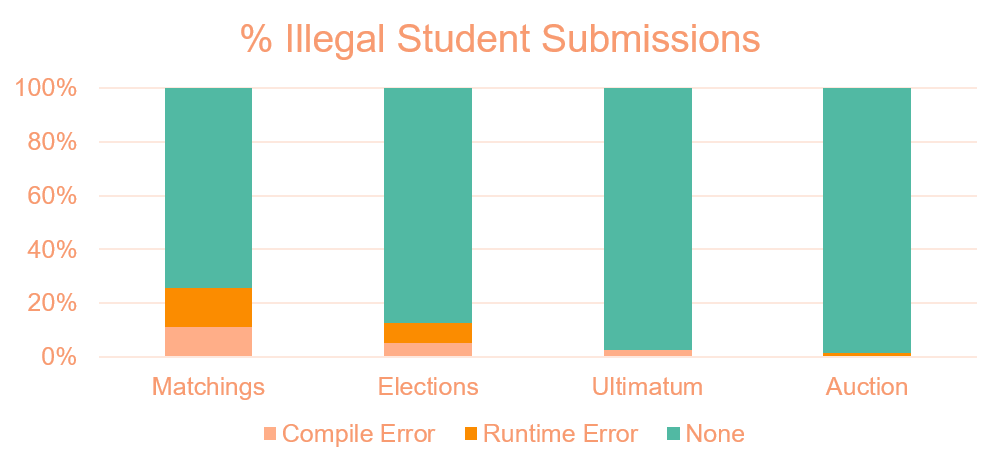
\includegraphics[width=0.75\linewidth]{illegal.png}
  \caption{Illegal submission rate dropped as my extensions were deployed. (Table~\ref{table:illegal})}\label{fig:illegal}
\end{figure}

Student polling data gathered at multiple points during the semester confirms that student engagement with newly released tools coincided with decreased rates of illegal submissions.
After the first two strategy design exercises, during which only the handout was provided, 68 of 74 respondents (out of 142 enrolled students) reported having used the handout to test their strategies~\cite{survey12}.
TODO student usage 34

Through this work, I have improved student and instructor experiences.
In addition to the data gathered above, I verified this achievement by surveying the current students of COS 445 under the supervision of Professor Weinberg.
In addition to usage data referenced above, survey respondents also evaluated their subjective rating for how useful the provided framework was in the design of their strategies.
TODO student rating 12 34

In order to evaluate instructor experiences, I reached out to Professor Weinberg for comment:
\begin{displayquote}
Andrew: What are your thoughts on how well the strategy design exercises have gone this year? Specifically, I'm interested in your satisfaction with the implementations and software, and the amount of instructor time and frustration spent.

Professor Weinberg: We have \textbf{significantly} improved instructor involvement. I didn't actually touch any of the software directly, so I don't know how to comment on that. But I felt like the challenges mostly ran themselves. We talked briefly to set it up. We talked briefly to decide how to grade, and I didn't have to answer any technical questions for students in between.
\end{displayquote}
My own experience an undergraduate course assistant using the framework I have developed in this work corroborates this claim: this project has led to better course experiences for all involved.

\section*{Conclusions and Future Work}
Through this work, my goal has been to improve the quality of present and future computer science theory education, from the perspectives of both the students and faculty associated with COS 445.

Student and instructor feedback indicates that my work has supported high quality strategy design exercises in the current Spring 2018 offering of COS 445.
Ease of development and grading of the later assignments in the course confirms that I made substantial progress in simplifying and automating the instructor experience.
Low rates of illegal student submissions confirm that my work has allowed students to focus on core assignment content without experiencing undue difficulties with assignment structure or available tooling.
I have achieved my goals in the present time-frame.

I intend to continue to use these tools as a returning undergraduate course assistant when this course is taught in Spring 2019.
However, I will graduate at the end of that semester and will be unavailable in subsequent offerings of COS 445.
I cannot yet measure my success at preventing this work from being repeated in any future year, but Professor Weinberg has confirmed that these resources will be provided to future course staff tasked with operating the strategy design exercises.

In Spring 2019, as supported within my existing framework, I will further simplify and automate the assignments.
While currently assignments are distributed independently, so no code may be shared between assignments, I will revise assignments to share one implementation of the handout post-processor and auto-grader post-processor.
This will complicate the assignment handout process slightly, but will simplify code reuse and iteration.
Earlier assignments were built off of earlier versions of the infrastructure and will need to be modified where they differ from newer versions when they are reused, but sharing code between assignments will prevent this inconsistency from developing again.

Recently, I became aware of a Java interface for loading classes at run time.
This technology, called ClassLoader~\cite{classloader}, was implemented in the Spring 2014 handout code.
I was unable to use ClassLoaders initially because I did not gain access to the Spring 2014 code until later in the semester.
This simple modification will eliminate Python dependency currently required by \texttt{formatBase.py} and allow students to better understand and modify handout simulation code.

Though few other universities currently teach courses in algorithmic game theory as undergraduate computer science, the field is growing and such courses will inevitably become more common.
As they do, they will look to COS 445 for resources, along with Stanford CS 269I, C.M.U.\ 15--196, and Harvard CS 136.
It is my hope that my code could be understood and assigned such courses, with modification to suit the topics covered.

\section*{Acknowledgments}
First of all, I would like to thank Professor Weinberg for his leadership in designing the written specifications and grading rubrics for the strategy design exercises, and for his dedication to teaching and organizing COS 445.
His dedication to the course engaged me as a student last year and was invaluable to my work this year.
I would like to thank Cyril Zhang for his work developing the implementation of the strategy design exercises I completed as a student, which inspired and served as a basis for this work.
Thanks to J\'er\'emie Lumbroso for providing me with the University-owned GitHub workspace in which my project has been stored in order to preserve it for future semesters of COS 445.

By grading student write-ups for strategy design exercises, Leila Clark, Wei Hu, Heesu Hwang, Dylan Mavrides, Andreea M\u{a}g\u{a}lie, Divyarthi Mohan, Ariel Schvartzman, Matheus Venturyne, and Evan Wildenhain provided me feedback about the quality of the handouts produced from my work and passed along student feedback.
These details provided crucial insights as to the clarity of the resources I have developed and allowed me to provide targeted documentation where my code was unclear.
Thanks also to all those students of COS 445 Spring 2018 for their feedback on the assignments used in the course, which informed my development of this project.

I created this work within the framework of Professor Dave Walker's Independent Work Seminar, I.W.\ 09: ``You Be The Prof''.
Professor Walker kept me organized and on schedule, and his guidance helped me identify and describe the topic of this work.
I also appreciate the feedback I received throughout the semester from my peers in Professor Walker's seminar, Noah Beattie-Moss, Mel Shu, Greg Umali, and Alex Xu.

I would like to thank Leila Clark and Kate Frain for their assistance revising this paper, and for their patience with my creative comma usage.
Kate also rescued me in my darkest hours with the delivery of hot chocolate.

\section*{Ethics}
Where there was potential for overlap between my role as an undergraduate course assistant for COS 445 and my development of this project, I have ensured that no hours were billed for work which I have described as a part of my independent work above.
Thus, I am not being awarded both payment as a course assistant and credit as an enrolled student for the same actions.
Though students completed assignments developed from and optionally provided feedback for these assignments while enrolled in COS 445, these interactions were overseen and approved by Professor Weinberg.
This paper represents my own work in accordance with university regulations.

\medskip
\singlespacing{}
\printbibliography[]

\newpage
\begin{appendices}
  \appendixpage{}
  \section{\texttt{writeGrades} demonstrates modularity in post-processing}\label{appendix:writeGrades}
\begin{minted}{java}
    public static void writeGrades () {
        final int numTrials = 1;
        //R netids[{0}] = "{netID}";//
        // defaults as specified in assignment handout PDF
        final double S = 100, T = 100, W = 10;
        // Compute x_i
        double[] oneEachTrials = oneEachTrials(100, S, T, W);

        // Instructor strategies
        List<Class<? extends Student>> ourStrats =
            new ArrayList<Class<? extends Student>>();
        ourStrats.add(Student_REDACTED.class);
        // a total of twelve such lines like the above line
        double[] winsToPoints = new double[]{
            0, 0.5, 1.0, 1.2, 1.5, 1.8, 2, 3, 3.5, 4.0, 4.5, 4.8, 5
        };
        // Compute \sum_j \delta_{x_i > y_j} for all i
        int[] wins = new int[N];
        for (Class<? extends Student> strat : ourStrats) {
            double[] res = withExtraTrials(strat, numTrials, S, T, W);
            for (int i = 0; i < N; ++i) {
                if (res[i] > res[N]) {
                    ++wins[i];
                }
            }
        }
        // Output grades as CSV
        System.out.println("netID,points");
        for (int i = 0; i < N; ++i) {
            System.out.println(netids[i]
                               + ","
                               + Double.toString(oneEachTrials[i])
                               + ","
                               + Double.toString(winsToPoints[wins[i]]));
        }
    }
\end{minted}
  \newpage
  \section{\texttt{formatBase.py} was used to automatically reconfigure the strategies to be simulated}\label{appendix:formatBase}
\begin{minted}{python}
import csv
import sys


def main():
    """
    Formats the standard input to standard output.
    Replaces lines of the form [\s]*//R(.*)//[\s]* with a line for every
    row of data.csv with the central string formatted according to the
    row of data.csv. Replaces lines of the form [\s]*//L(.*)//[\s]* with
    the central string formatted with the number of rows.
    """
    if len(sys.argv) != 2:
        sys.exit("Usage: {} [data.csv] < [ClassBase.java] > [Class.java]"
                 .format(sys.argv[0]))

    with open(sys.argv[1]) as f:
        reader = csv.DictReader(f, skipinitialspace=True)
        rows = [{k: v for k, v in row.items()} for row in reader]

    for line_ in sys.stdin:
        line_ = line_.rstrip()
        line = line_.strip()
        if line.startswith("//L") and line.endswith("//"):
            print(line[3:-2].format(len(rows)))

        elif line.startswith("//R") and line.endswith("//"):
            for i, vals in enumerate(rows):
                print(line[3:-2].format(i, **vals))

        else:
            print(line_)


if __name__ == "__main__":
    main()

\end{minted}

  \newpage
  \section{\texttt{students.csv} provides an example configuration for \texttt{formatBase.py}}\label{appendix:students}
\begin{Verbatim}
netID
random
random
random
random
random
random
random
random
random
random
favorites
favorites
favorites
favorites
favorites
favorites
favorites
favorites
favorites
favorites
favorites
favorites
favorites
favorites
favorites
\end{Verbatim}

\newpage
\section{COS 333 Spring 2017 Survey Data}\label{appendix:cos333sp17}
Thanks to Professor Kernighan for providing my independent work seminar with this data.
\begin{Verbatim}[fontsize=\scriptsize]
181 responses
Class
 2017 10
 2018 89
 2019 82
Major
 COS 148        ELE 12         ORF 4          WWS 2          MAT 2          ECO 2         
 SPA 1          POL 1          PHI 1          HIS 1          GER 1          AST 1         
 ARC 1          AB 1           A.B. 1        
Certificate  23
Course
 C217 178       C226 175       C126 161       C326 36        C318 21        C461 8        
 C418 1         C320 1        
Fluent
 Java 133       C 61           Python 32      Javascript 17  HTML 9         OCaml 6       
 Matlab 6       R 5            Swift 4        English 4      CSS 4          C++ 4         
 C# 4           PHP 3          Verilog 2      Ruby 2         Assembly 2     X86-64 1      
 TypeScript 1   Scala 1        SQL 1          SCSS 1         Perl 1         Ofcourse 1    
 NodeJavascrip  Haskell 1      Greek 1        ChucK 1       
Cope:
 Python 41      C 37           HTML 24        Javascript 17  Java 15        CSS 13        
 OCaml 12       Matlab 10      C++ 10         PHP 9          Ruby 8         C# 8          
 Swift 7        Verilog 6      SQL 6          R 6            MySQL 3        Assembly 3    
 x86-64 2       VB 2           Rails 2        Perl 2         Go 2           Fortran 2     
 3 1            x86 1          up 1           seem 1         regular 1      only 1        
 not 1          most 1         mark 1         little 1       learn 1        languages 1   
 iOS-Swift 1    extremely 1    but 1          bit 1          X86 1          WebGL 1       
 VBA 1          Scheme 1       SCSS 1         Rust 1         React-Native   React 1       
 OpenGL 1       Objective 1    N 1            Lisp 1         LaTeX 1        I 1           
 Haskell 1      Common 1       Coffeescript   Clojure 1      Can 1          Bash 1        
 Arabic 1       Android 1      AVR 1          AMPL 1         - 1           
More:
 Python 42      Javascript 33  Ruby 23        C++ 22         Swift 20       SQL 17        
 PHP 17         HTML 16        Go 14          CSS 9          Perl 5         Haskell 5     
 C# 5           C 5            Scala 4        iOS 3          Rust 3         Objective 3   
 OCaml 3        languages 2    functional 2   else 2         anything 2     React 2       
 MySQL 2        Lisp 2         Erlang 2       Clojure 2      Android 2      what's 1      
 web 1          to 1           them 1         or 1           often 1        of 1          
 mobile 1       maybe 1        lot 1          language? 1    know 1         jQuery 1      
 in 1           front-end 1    for 1          everything 1   especially 1   emacs 1       
 else. 1        don't 1        dev 1          css 1          app 1          Super 1       
 Solidity 1     Scripts 1      R 1            Prolog 1       Or 1           Open 1        
 Objective-C 1  Not 1          NodeJavascrip  Mongo 1        Mobile 1       Maybe 1       
 Matlab 1       Lua 1          Julia 1        JQuery 1       Idris 1        IOS 1         
 I 1            FORTRAN 1      F# 1           Everything 1   Dev 1          D 1           
 Coq 1          CoffeeScript   Chinese 1      Arabic 1       App 1          Any 1         
 All 1          .NET 1        
Unix      48  37  59  34
Win       86  35  40  16
Mac       78  25  45  30
iOS      126  25  21   5
Android  107  40  25   7
Win 55, Mac 134, Linux 12
iPhone 126, Android 55, Other 0
181 responses
\end{Verbatim}

\newpage
\section{COS 333 Spring 2018 Survey Data}\label{appendix:cos333sp18}
Thanks to Professor Kernighan for providing my independent work seminar with this data.
\begin{Verbatim}[fontsize=\scriptsize]
Names 103
2018 14
2019 25
2020 64
 103
Majors:
   cos 82
   ele 6
   orf 5
   phy 2
   mae 2
   eco 2
   mol 1
   mat 1
   geo 1
   ast 1
Certif 17
126 93
217 100
226 102
318 2
320 
326 11
418 3
425 
435 1
436 
461 12
Unix    lots 13 some 55 little 22 none 12
Win lots 19 some 32 little 16 none 33
MacOSX  lots 20 some 29 little 14 none 39
iOS lots 7 some 11 little 16 none 67
Android lots 8 some 14 little 24 none 54
PCwin 42
PClinux 9
PCmac 66
iPhone 64
Android 40
other 0
Fluent
   java 91 c 67 python 29 javascript 8 c++ 8 r 7 matlab 6 html 6 ocaml 4
   css 4 react 3 swift 2 asm 2 wolfram 1 verilog 1 stata 1 sql 1 scala 1
   ruby 1 php 1 objective-c 1 native 1 latex 1 julia 1 jquery 1 fortran 1
   bash 1
Cope
   python 35 c 30 javascript 21 r 12 c++ 12 java 11 matlab 9 html 9 sql 6
   ocaml 6 php 5 css 5 swift 4 go 3 asm 3 verilog 2 ruby 2 objective-c 2
   lua 2 c# 2 xml 1 throwback 1 stata 1 scala 1 roughly 1 rails 1 other 1
   mysql 1 know 1 julia 1 i 1 haskell 1 fortran 1 f# 1 c#.net 1 at&t 1
   ample 1 VB 1 64 1
More
   javascript 38 python 37 c++ 22 html 17 sql 14 ruby 11 go 11 swift 8
   css 8 c# 7 scala 5 react 3 perl 3 haskell 3 web 2 php 2 other 2 c 2
   them 1 stack 1 rust 1 reactjavascript 1 rails 1 r 1 others 1 of 1
   ocaml 1 objective-c 1 native 1 mysql 1 my 1 missing 1 mean 1 matlab 1
   many 1 list 1 latex 1 languages 1 kotlin 1 java 1 is 1 ios 1 http 1
   html5 1 hadoop 1 golang 1 git 1 from 1 frameworks 1 experience 1
   everything 1 etc.  1 essential 1 else 1 databases 1 clojure 1 awk 1
   application 1 android 1
\end{Verbatim}

\newpage
\section{Data Tables}\label{appendix:tables}

\begin{table}[!h]
  \centering
  \begin{tabular}{l|c c c}  & Design& Build& Grade\\
    \hline
    1. Matching& 5& 15& 20\\
    2. Election& 5& 10& 15\\
    3. Ultimatum& 5& 5& 5\\
    4. Auction& 5& 1.5& 5
  \end{tabular}
  \caption{Instructor time usage per assignment (hours)}\label{table:time}
\end{table}
This data is approximate and based on revision logs reviewed later in the semester.
Instructor time usage for early assignments includes framework development not performed by course staff where that work was necessary for the completion of the assignment development and grading.

\begin{table}[!h]
  \centering
  \begin{tabular}{l|c c c} & Compile Error& Runtime Error& None\\
    \hline
    1. Matchings& 9& 12& 61\\
    2. Elections& 4& 6& 70\\
    3. Ultimatum& 2& 0& 75\\
    4. Auction& 0& 1& 75
  \end{tabular}
  \caption{Incidence of illegal submissions per assignment}\label{table:illegal}
\end{table}
I accessed this data in my role as an undergraduate course assistant and received Professor Weinberg's approval to include it in this paper.

\end{appendices}
\end{document}

%  LocalWords:  Wonnacott LocalWords writeGrades modularity Xu Zhang
%  LocalWords:  Wildenhain baselinestretch matchings cryptocurrencies
%  LocalWords:  cryptocurrency blockchain Zhang's Yonatan Braverman
%  LocalWords:  CAS PHP leaderboard iteratively programatically Ocaml
%  LocalWords:  nullable unmodifiable NotNull Kernighan Shapley myBid
%  LocalWords:  dailyValue myPayment addResults getBid sed CSV py hbt
%  LocalWords:  formatBase netID oneEachTrial runTrial withExtraTrial
%  LocalWords:  clazz ReflectiveOperationException printStackTrace Hu
%  LocalWords:  incentivized Makefile modularization cron emie Heesu
%  LocalWords:  customizable extensibility ClassLoaders Lumbroso Shu
%  LocalWords:  Hwang Mavrides Andreea Divyarthi Mohan Schvartzman
%  LocalWords:  Matheus Venturyne Beattie Frain Umali numTrials strat
%  LocalWords:  netids oneEachTrials ourStrats ArrayList winsToPoints
%  LocalWords:  withExtraTrials toString Naamad
